\documentclass[10pt,a4paper]{article}
\usepackage[margin=1.65 cm,top=1.4 cm,bottom=1.5 cm]{geometry}
\usepackage[T1]{fontenc}
\usepackage[utf8]{inputenc}
\usepackage{lmodern,microtype,booktabs,tabularx,array,amsmath,graphicx,xcolor,colortbl,hyperref,enumitem,fancyhdr}
\definecolor{navy}{HTML}{183B56}\definecolor{teal}{HTML}{187F80}
\hypersetup{colorlinks=true,urlcolor=teal,linkcolor=navy,pdftitle={Thesis Progress Update: Batch Scaling and Classifier Comparison},pdfauthor={Eren Olmez}}
\setlength{\parindent}{0 pt}\setlength{\parskip}{4 pt}\setlength{\emergencystretch}{2 em}
\renewcommand{\arraystretch}{1.12}
\setlist[itemize]{leftmargin=1.2 em,itemsep=1 pt,topsep=2 pt}
\pagestyle{fancy}\fancyhf{}\fancyhead[L]{\small\color{navy}Energy-efficient input-based model routing}
\fancyhead[R]{\small 24 November 2026}\fancyfoot[C]{\small\thepage}\setlength{\headheight}{13 pt}
\newcommand{\heading}[1]{\section*{\color{navy}#1}}
\newcommand{\smallcap}[1]{{\footnotesize\color{navy}#1}\par}
\newcommand{\missing}{\textemdash}
\newcommand{\newbatch}[2]{ & \textbf{#1} & \textbf{#2\%} & \missing & \missing & \missing & \missing\\}
% The routed comparison is the canonical meeting report.
\providecommand{\RoutedProgressUpdate}{1}
\begin{document}
\begin{center}
{\Large\bfseries\color{navy}Thesis Progress Update}\\[3 pt]
{Eren Olmez}\\{24 November 2026}
\end{center}\vspace{-8 pt}

\ifdefined\RoutedProgressUpdate
\heading{1. Does the end-to-end router plateau?}
\textbf{What changed?} The TinyCNN still chooses one of 213 classifiers for the entire batch. We now keep the most frequently selected classifiers resident on the GPU, ranked using only the 2,000 calibration images for each batch size. The resident count is limited by available memory, not a fixed cap. An uncached choice can still run on demand. All qualifying passes reproduced the original predictions exactly.

\def\RoutedResnetRows{%
8 & 85.05\% & 6.74 & 0.842 & 63.21 & 85.85\% & 6.86 & 0.858 & 65.84\\%
16 & 84.92\% & 8.79 & 0.549 & 40.86 & 85.85\% & 9.24 & 0.578 & 43.40\\%
32 & 84.96\% & 13.55 & 0.424 & 30.57 & 85.85\% & 14.33 & 0.449 & 32.81\\%
64 & 84.02\% & 21.21 & 0.333 & 24.25 & 85.85\% & 26.88 & 0.422 & 30.69\\%
128 & 84.02\% & 38.48 & 0.304 & 22.12 & 85.85\% & 52.14 & 0.412 & 30.46\\%
}

\begin{center}\small
\begin{tabular}{@{}rrrrrrrrr@{}}\toprule
 & \multicolumn{4}{c}{Batch router} & \multicolumn{4}{c}{Fixed ResNet101 FP16}\\
\cmidrule(lr){2-5}\cmidrule(lr){6-9}
Batch & Test acc. & ms/batch & ms/image & mJ/image & Test acc. & ms/batch & ms/image & mJ/image\\
\midrule
\RoutedResnetRows
\bottomrule\end{tabular}
\end{center}
\smallcap{Medians of qualifying passes over 10,000 CIFAR-100 test images; energy is GPU-only. At batches 8/16/32/64/128 the repeat counts were 1/3/3/2/3 for the router and 1/1/2/2/2 for ResNet101. Each pass warmed up for at least 30 seconds and 50 batches, then cooled to at most 65 degrees Celsius before timing without clearing the classifier cache. Both qualifying batch-8 passes used a 64-degree gate.}

\begin{center}\vspace{-2pt}
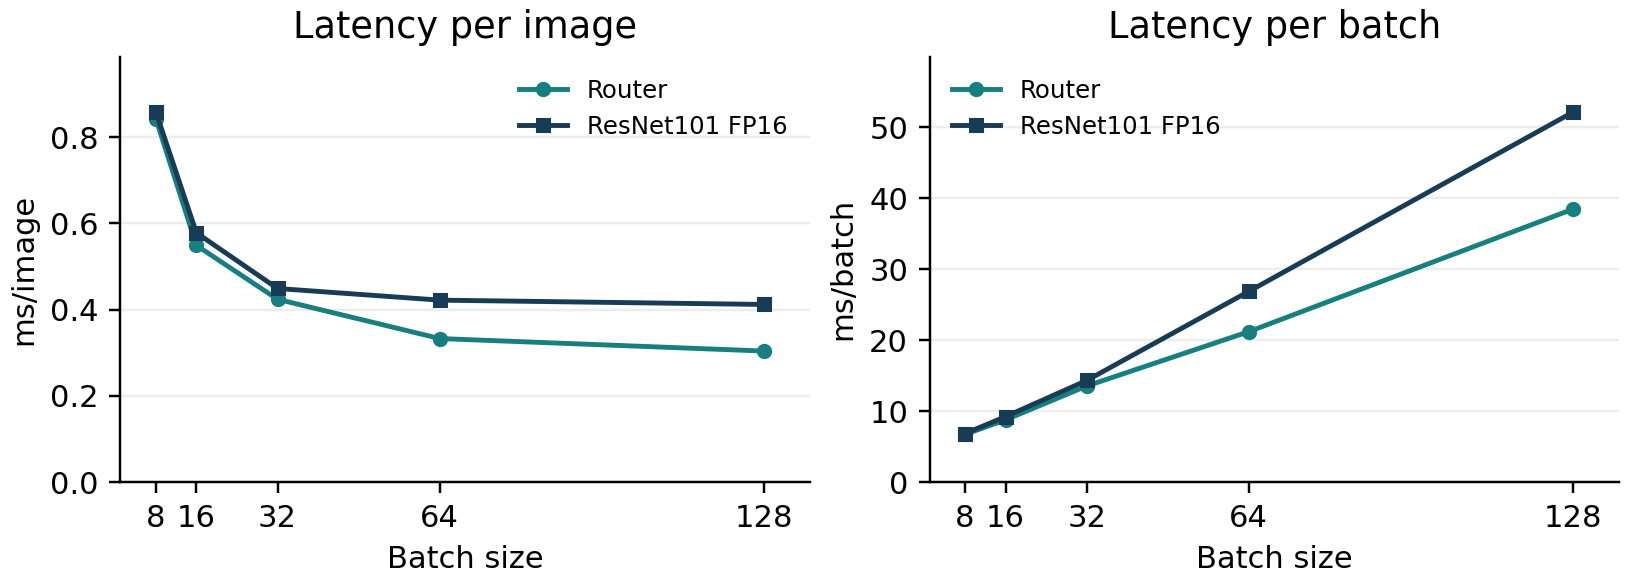
\includegraphics[width=.93\linewidth]{router-resnet101-latency.png}\\[-2pt]
\end{center}\vspace{-4pt}
\smallcap{Only qualifying table values are plotted. Time per batch includes the shorter final batch when present.}

\textbf{Did residency reduce reloads?} Calibration chose four distinct models at batch 8, three at 16, and two at each of 32, 64, and 128. All fit while leaving at least 1 GiB free. Qualifying passes had no timed disk reads. Batch 32 loaded one extra classifier from RAM per pass; batches 16, 64, and 128 needed no timed GPU loads.

\textbf{What is the trade-off?} The router was faster per image than fixed ResNet101 at every tested batch size in these measurements, but less accurate. At batch 8 the latency difference was only 0.016 ms per image, with one qualifying repeat for each path, so it is not a reliable speedup estimate. The routed batch-64 and batch-128 scores both equal 84.02\%, but the predictions differed: each got 8,402 images right, not necessarily the same images.

\else
\heading{1. Batch scaling on the PC}
This update extends the fixed-classifier comparison from the 6 November report to batches 8 and 16. The two unpruned FP16 TensorRT engines and their original optimization profiles were retained. The table separates test accuracy from latency and GPU energy, and keeps the two input/output boundaries separate.

\textbf{What changed at batches 8 and 16?}
Both new batch sizes reproduced the archived top-1 accuracy: 85.85\% for ResNet101 and 82.71\% for EfficientNet-B0. Equal scores do not by themselves establish identical predictions on every image.

\begin{center}\small
\begin{tabular}{@{}lrrrrrr@{}}\toprule
 & & & \multicolumn{2}{c}{GPU-resident input} & \multicolumn{2}{c}{Host input to host logits}\\
\cmidrule(lr){4-5}\cmidrule(lr){6-7}
FP16 classifier & Batch & Test acc. & ms/image & GPU mJ/image & ms/image & GPU mJ/image\\
\midrule
ResNet101 \newbatch{8}{85.85}
\newbatch{16}{85.85}
 & 32 & 85.85\% & 0.3355 & 23.170 & 0.3632 & 25.509\\
 & 64 & 85.85\% & 0.3265 & 23.162 & 0.3518 & 24.313\\
 & 128 & 85.85\% & 0.3190 & 22.125 & 0.3457 & 23.512\\
\addlinespace[2pt]
EfficientNet-B0 \newbatch{8}{82.71}
\newbatch{16}{82.71}
 & 32 & 82.71\% & 0.1384 & 9.895 & 0.1701 & 12.140\\
 & 64 & 82.71\% & 0.1242 & 8.862 & 0.1629 & 11.340\\
 & 128 & 82.71\% & 0.1164 & 8.046 & 0.1456 & 10.497\\
\bottomrule\end{tabular}
\end{center}
\smallcap{Top-1 accuracy uses all 10,000 CIFAR-100 test images. Original timing and GPU-only energy medians use 128 fixed validation inputs per cycle and three windows per model, boundary and batch. Dashes denote unmeasured timing or energy.}

\textbf{Why did the timing run stop if the GPU is warmed up?}
The protocol first requires at least 15 seconds of cooldown and a temperature of at most 55 degrees Celsius, with no thermal slowdown flag. It then runs at least one second of model-specific warm-up immediately before the timed window. This gives each repeat a comparable starting condition without including cold-start inference in its timer. The new run could not clear the cooldown gate within 180 seconds, so it collected no accepted timing windows. The separate accuracy run was unaffected.

\textbf{What can be concluded now?}
The original GPU-resident results still show improvement from batch 32 to 128: latency and GPU energy dropped by 4.92\% and 4.51\% for ResNet101 and by 15.91\% and 18.69\% for EfficientNet-B0. This is a fixed-model result; it does not explain the old routed plateau. The next matched timing pass will use batches 8, 16 and a repeat of 32 to check comparability with November 6.
\fi

\newpage
\heading{2. HPC classifier sweep and PC comparison}
The frozen scratch sweep covers eight architectures, 72 recipes per architecture, three seeds per recipe and 200 epochs per case. The verified W\&B snapshot recorded \textbf{1,629/1,728 complete cases (94.27\%)} and \textbf{327,184/345,600 recorded epochs (94.67\%)}. W\&B showed 99 failed or crashed records and no run marked running; this does not establish the Slurm queue state.

\begin{center}\small
\begin{tabular}{@{}lrrrrr@{}}\toprule
 & & \multicolumn{2}{c}{HPC scratch, 32px} & \multicolumn{2}{c}{Historical PC FP32, 128px}\\
\cmidrule(lr){3-4}\cmidrule(lr){5-6}
Architecture & Case / seed & Best val. & Test & Val. & Test\\
\midrule
ResNet101             & 0139 / 48 & 81.82\% & 81.01\% & 85.88\% & 85.80\%\\
ResNet34              & 0329 / 48 & 81.66\% & 79.86\% & 82.98\% & 81.82\%\\
ResNet50              & 0314 / 42 & 81.26\% & 79.97\% & 83.94\% & 84.39\%\\
ResNet18              & 0312 / 42 & 80.12\% & 78.28\% & 79.16\% & 79.16\%\\
ShuffleNetV2 x1.0     & 0415 / 42 & 75.56\% & 73.46\% & 75.72\% & 75.64\%\\
EfficientNet-B0       & 1678 / 48 & 73.30\% & 72.31\% & 83.14\% & 82.73\%\\
MobileNetV3 Large     & 0237 / 48 & 72.52\% & 71.26\% & 82.04\% & 81.34\%\\
MobileNetV3 Small     & 0228 / 45 & 64.42\% & 62.48\% & 61.82\% & 62.38\%\\
\bottomrule\end{tabular}
\end{center}
\smallcap{Each HPC row represents the highest observed validation accuracy from one completed run, not a three-seed recipe ranking. Both validation sets contain 5,000 images but use different splits. Both test columns use all 10,000 official CIFAR-100 test images.}

\textbf{What settings did the scratch leaders use?}
All eight used batch size 128, cosine decay and CutMix ($\alpha=1$, probability 0.5). Seven used SGD (momentum 0.9): initial learning rate 0.10 except ResNet101 (0.03) and ShuffleNetV2 (0.20). SGD weight decay was $5\times10^{-4}$ for the ResNets and $10^{-4}$ for MobileNetV3 and ShuffleNetV2. EfficientNet-B0 used AdamW (learning rate 0.003, weight decay 0.05).

\textbf{What does this table compare?}
The first table compares two existing model banks on the same official test set: scratch HPC models with CIFAR-adapted stems in PyTorch FP32 at native 32px, and historical ImageNet-initialized PC models in TensorRT FP32 at 128px. The checkpoints were selected on validation, but the banks used different validation splits and training recipes.

\subsection*{ImageNet-pretrained HPC comparison}
The second table compares validation accuracy on the same HPC classifier split (40,000 training and 5,000 validation images) and test accuracy on the official holdout. For each architecture, the two input sizes reuse one scratch recipe and seed and start from the same ImageNet-initialized weights. W\&B recorded \textbf{16/16 cases and 3,200/3,200 epochs complete (100\%)}.

\begin{center}\small
\begin{tabular}{@{}lrrrrrr@{}}\toprule
 & \multicolumn{2}{c}{Scratch 32px} & \multicolumn{2}{c}{Pretrained 32px} & \multicolumn{2}{c}{Pretrained 128px}\\
\cmidrule(lr){2-3}\cmidrule(lr){4-5}\cmidrule(lr){6-7}
Architecture & Best val. & Test & Best val. & Test & Best val. & Test\\
\midrule
ResNet101          & 81.82\% & 81.01\% & 60.64\% & 59.27\% & 86.24\% & 84.38\%\\
ResNet34           & 81.66\% & 79.86\% & 66.54\% & 65.01\% & 81.26\% & 80.28\%\\
ResNet50           & 81.26\% & 79.97\% & 69.12\% & 67.84\% & 82.34\% & 81.37\%\\
ResNet18           & 80.12\% & 78.28\% & 65.50\% & 63.49\% & 80.84\% & 79.56\%\\
ShuffleNetV2 x1.0  & 75.56\% & 73.46\% & 56.38\% & 54.96\% & 76.30\% & 75.69\%\\
EfficientNet-B0    & 73.30\% & 72.31\% & 26.96\% & 25.72\% & 82.62\% & 81.10\%\\
MobileNetV3 Large  & 72.52\% & 71.26\% & 54.94\% & 53.91\% & 82.90\% & 81.37\%\\
MobileNetV3 Small  & 64.42\% & 62.48\% & 39.08\% & 40.00\% & 72.30\% & 71.18\%\\
\bottomrule\end{tabular}
\end{center}
\textbf{Why might 128px work better here?}
ImageNet weights provide learned visual features. Upsampling adds no image detail, but gives the pretrained network more spatial positions after early downsampling, which may help it reuse those features. At 128px, seven of eight models beat scratch on validation and all eight beat scratch on test; at 32px none did. The pretrained models use PC stems rather than CIFAR-adapted stems, so the scratch comparison does not isolate pretraining.

\smallcap{All test scores in the second table are PyTorch FP32 top-1 accuracy over 10,000 official CIFAR-100 images. Checkpoints were selected on validation before test evaluation. Pruning uses only the scratch checkpoints.}

\smallcap{Sources: \href{https://github.com/erenolmez/energy-efficient-edge-ai/blob/9dc335f/progress_reports/2026-11-06/progress_report.tex}{6 November progress report}; \href{https://github.com/erenolmez/energy-efficient-edge-ai/blob/9dc335f/progress_reports/2026-10-29/runtime_explanations.tex}{29 October runtime follow-up}; archived PC TensorRT results; HPC W\&B snapshots; held-out evaluation job 2141241.}
\ifdefined\RoutedProgressUpdate
\newpage
\heading{3. After pruning, which classes are easiest and hardest?}
Each requested pruning level (10--90\%) starts from the best-validation 32px HPC scratch checkpoint. Fine-tuning used Adam at 0.001 and validation-based stopping (10--25 epochs). Selected checkpoints were tested in PyTorch FP32 on all 10,000 official CIFAR-100 images (100 per class). \textbf{All 63 runs are complete (100\%)}. ShuffleNetV2 is not supported by this structural pruner.

\textbf{What changes at 10\% requested pruning?}
\vspace{-4pt}\begin{center}\small\setlength{\tabcolsep}{5pt}
\begin{tabularx}{\linewidth}{@{}lrrXX@{}}\toprule
Architecture & Unpruned test & p10 test & p10 worst class & p10 best class(es)\\
\midrule
ResNet18 & 78.28\% & 71.38\% & seal (26\%) & motorcycle (97\%)\\
ResNet34 & 79.86\% & 71.81\% & forest (39\%) & motorcycle (98\%)\\
ResNet50 & 79.97\% & 73.35\% & seal (38\%) & motorcycle (96\%)\\
ResNet101 & 81.01\% & 67.29\% & man (27\%) & orange (98\%)\\
MobileNetV3 Small & 62.48\% & 55.48\% & man (15\%) & skyscraper (89\%)\\
MobileNetV3 Large & 71.26\% & 63.45\% & woman (24\%) & road (94\%)\\
EfficientNet-B0 & 72.31\% & 65.02\% & girl (30\%) & motorcycle / orange (95\%)\\
\bottomrule\end{tabularx}
\end{center}\vspace{-4pt}
\smallcap{All scores are test accuracy. The p10 overall accuracy drop ranges from 6.62 percentage points (ResNet50) to 13.72 points (ResNet101). Requested pruning is not the measured reduction in parameters or multiply-accumulate operations.}

\textbf{How does the weakest class change as pruning increases?}
\vspace{-4pt}\begin{center}\small\setlength{\tabcolsep}{5pt}
\begin{tabular}{@{}l*{9}{r}@{}}\toprule
Requested pruning (\%) & 10 & 20 & 30 & 40 & 50 & 60 & 70 & 80 & 90\\
\midrule
ResNet18 & \cellcolor{teal!16}26 & \cellcolor{teal!19}30 & \cellcolor{teal!25}40 & \cellcolor{teal!11}17 & \cellcolor{teal!18}29 & \cellcolor{teal!20}31 & \cellcolor{teal!12}19 & \cellcolor{teal!8}12 & \cellcolor{teal!3}5\\
ResNet34 & \cellcolor{teal!25}39 & \cellcolor{teal!25}40 & \cellcolor{teal!21}34 & \cellcolor{teal!25}40 & \cellcolor{teal!25}40 & \cellcolor{teal!19}30 & \cellcolor{teal!11}18 & \cellcolor{teal!9}14 & \cellcolor{teal!6}10\\
ResNet50 & \cellcolor{teal!24}38 & \cellcolor{teal!19}30 & \cellcolor{teal!16}26 & \cellcolor{teal!22}35 & \cellcolor{teal!21}34 & \cellcolor{teal!18}28 & \cellcolor{teal!22}35 & \cellcolor{teal!13}21 & \cellcolor{teal!13}21\\
ResNet101 & \cellcolor{teal!17}27 & \cellcolor{teal!19}30 & \cellcolor{teal!21}33 & \cellcolor{teal!16}25 & \cellcolor{teal!21}33 & \cellcolor{teal!22}35 & \cellcolor{teal!11}18 & \cellcolor{teal!8}12 & \cellcolor{teal!4}6\\
MobileNetV3 Small & \cellcolor{teal!9}15 & \cellcolor{teal!12}19 & \cellcolor{teal!14}23 & \cellcolor{teal!7}11 & \cellcolor{teal!12}19 & \cellcolor{teal!4}7 & \cellcolor{teal!5}8 & \cellcolor{teal!3}4 & \cellcolor{teal!6}10\\
MobileNetV3 Large & \cellcolor{teal!15}24 & \cellcolor{teal!17}27 & \cellcolor{teal!17}27 & \cellcolor{teal!13}21 & \cellcolor{teal!14}23 & \cellcolor{teal!11}18 & \cellcolor{teal!3}5 & \cellcolor{teal!9}14 & \cellcolor{teal!11}18\\
EfficientNet-B0 & \cellcolor{teal!19}30 & \cellcolor{teal!13}20 & \cellcolor{teal!21}33 & \cellcolor{teal!17}27 & \cellcolor{teal!12}19 & \cellcolor{teal!13}20 & \cellcolor{teal!5}8 & \cellcolor{teal!10}16 & \cellcolor{teal!0}0\\
\bottomrule\end{tabular}
\end{center}\vspace{-4pt}

\textbf{How does the strongest class change as pruning increases?}
\vspace{-4pt}\begin{center}\small\setlength{\tabcolsep}{5pt}
\begin{tabular}{@{}l*{9}{r}@{}}\toprule
Requested pruning (\%) & 10 & 20 & 30 & 40 & 50 & 60 & 70 & 80 & 90\\
\midrule
ResNet18 & \cellcolor{teal!61}97 & \cellcolor{teal!62}98 & \cellcolor{teal!60}95 & \cellcolor{teal!61}97 & \cellcolor{teal!60}95 & \cellcolor{teal!60}96 & \cellcolor{teal!59}93 & \cellcolor{teal!59}93 & \cellcolor{teal!58}92\\
ResNet34 & \cellcolor{teal!62}98 & \cellcolor{teal!60}96 & \cellcolor{teal!61}97 & \cellcolor{teal!60}95 & \cellcolor{teal!58}92 & \cellcolor{teal!60}95 & \cellcolor{teal!61}97 & \cellcolor{teal!57}91 & \cellcolor{teal!58}92\\
ResNet50 & \cellcolor{teal!60}96 & \cellcolor{teal!60}96 & \cellcolor{teal!60}96 & \cellcolor{teal!59}94 & \cellcolor{teal!59}94 & \cellcolor{teal!60}95 & \cellcolor{teal!60}95 & \cellcolor{teal!58}92 & \cellcolor{teal!57}91\\
ResNet101 & \cellcolor{teal!62}98 & \cellcolor{teal!59}94 & \cellcolor{teal!60}96 & \cellcolor{teal!60}95 & \cellcolor{teal!59}93 & \cellcolor{teal!59}94 & \cellcolor{teal!60}96 & \cellcolor{teal!55}87 & \cellcolor{teal!56}89\\
MobileNetV3 Small & \cellcolor{teal!56}89 & \cellcolor{teal!56}89 & \cellcolor{teal!57}90 & \cellcolor{teal!57}90 & \cellcolor{teal!56}89 & \cellcolor{teal!53}84 & \cellcolor{teal!53}84 & \cellcolor{teal!55}87 & \cellcolor{teal!57}91\\
MobileNetV3 Large & \cellcolor{teal!59}94 & \cellcolor{teal!59}93 & \cellcolor{teal!58}92 & \cellcolor{teal!59}93 & \cellcolor{teal!57}91 & \cellcolor{teal!57}91 & \cellcolor{teal!54}86 & \cellcolor{teal!54}86 & \cellcolor{teal!58}92\\
EfficientNet-B0 & \cellcolor{teal!60}95 & \cellcolor{teal!57}91 & \cellcolor{teal!59}93 & \cellcolor{teal!59}94 & \cellcolor{teal!58}92 & \cellcolor{teal!57}91 & \cellcolor{teal!57}90 & \cellcolor{teal!57}91 & \cellcolor{teal!55}88\\
\bottomrule\end{tabular}
\end{center}\vspace{-4pt}
\smallcap{Both tables use the same color scale for class test accuracy (\%). Class identities can change across levels. ResNet50 p90 reached 63.24\% overall test accuracy.}

\textbf{Where do models disagree most?}
ResNet50 and MobileNetV3 Small had the largest gaps: raccoon at p10 (86\% vs.\ 40\%) and turtle at p50 (79\% vs.\ 26\%). These gaps do not establish a routing benefit.

\textbf{Which class names change at higher pruning levels?}\par
{\footnotesize\setlength{\tabcolsep}{3pt}\renewcommand{\arraystretch}{1.05}
\newcommand{\classpair}[2]{\textcolor{navy}{#1}\newline #2}
\begin{tabularx}{\linewidth}{@{}l*{4}{>{\raggedright\arraybackslash}X}@{}}\toprule
Architecture & p30 & p50 & p70 & p90\\
\midrule
ResNet18 & \classpair{mountain}{bowl} & \classpair{motorcycle}{girl} & \classpair{orange}{girl} & \classpair{wardrobe}{mouse}\\
ResNet34 & \classpair{orange}{oak tree} & \classpair{apple}{man} & \classpair{motorcycle}{otter} & \classpair{orange / wardrobe}{otter}\\
ResNet50 & \classpair{motorcycle}{girl} & \classpair{motorcycle / orange}{woman} & \classpair{lawn mower}{bear} & \classpair{motorcycle}{otter}\\
ResNet101 & \classpair{orange}{otter} & \classpair{motorcycle / orange / wardrobe}{otter} & \classpair{wardrobe}{otter} & \classpair{motorcycle / plain}{otter}\\
MobileNetV3 Small & \classpair{apple / sunflower}{girl / seal} & \classpair{orange}{seal} & \classpair{sunflower}{beaver} & \classpair{sunflower}{otter}\\
MobileNetV3 Large & \classpair{wardrobe}{lizard} & \classpair{motorcycle / orange / road}{otter / seal} & \classpair{skyscraper}{woman} & \classpair{orange}{seal}\\
EfficientNet-B0 & \classpair{road}{seal / shark} & \classpair{road}{seal} & \classpair{wardrobe}{otter} & \classpair{orange}{otter}\\
\bottomrule\end{tabularx}\par}
\smallcap{Each cell lists the best class(es) in navy on top and the worst class(es) below. Slashes indicate ties. The heatmaps above give the scores.}

\newpage
\heading{Pruning: best and worst classes at every level}
For each architecture and requested pruning level, the \textcolor{navy}{best class is on top} and the worst class is below. Percentages are per-class accuracy on the official CIFAR-100 test set. A slash separates classes tied at the same accuracy.

{\small\setlength{\tabcolsep}{4pt}\renewcommand{\arraystretch}{1.12}
\newcommand{\classpair}[2]{\textcolor{navy}{#1}\newline #2}
\begin{tabularx}{\linewidth}{@{}l*{5}{>{\raggedright\arraybackslash}X}@{}}\toprule
Architecture & p10 & p20 & p30 & p40 & p50\\
\midrule
ResNet18 & \classpair{motorcycle (97\%)}{seal (26\%)} & \classpair{motorcycle (98\%)}{seal (30\%)} & \classpair{mountain (95\%)}{bowl (40\%)} & \classpair{wardrobe (97\%)}{bear (17\%)} & \classpair{motorcycle (95\%)}{girl (29\%)}\\
\addlinespace[3pt]
ResNet34 & \classpair{motorcycle (98\%)}{forest (39\%)} & \classpair{apple / motorcycle (96\%)}{otter (40\%)} & \classpair{orange (97\%)}{oak tree (34\%)} & \classpair{motorcycle / wardrobe (95\%)}{bear (40\%)} & \classpair{apple (92\%)}{man (40\%)}\\
\addlinespace[3pt]
ResNet50 & \classpair{motorcycle (96\%)}{seal (38\%)} & \classpair{skunk (96\%)}{seal (30\%)} & \classpair{motorcycle (96\%)}{girl (26\%)} & \classpair{motorcycle / palm tree (94\%)}{seal (35\%)} & \classpair{motorcycle / orange (94\%)}{woman (34\%)}\\
\addlinespace[3pt]
ResNet101 & \classpair{orange (98\%)}{man (27\%)} & \classpair{orange / palm tree (94\%)}{bear (30\%)} & \classpair{orange (96\%)}{otter (33\%)} & \classpair{skunk (95\%)}{man / seal (25\%)} & \classpair{motorcycle / orange / wardrobe (93\%)}{otter (33\%)}\\
\addlinespace[3pt]
MobileNetV3 Small & \classpair{skyscraper (89\%)}{man (15\%)} & \classpair{road (89\%)}{lizard (19\%)} & \classpair{apple / sunflower (90\%)}{girl / seal (23\%)} & \classpair{wardrobe (90\%)}{seal (11\%)} & \classpair{orange (89\%)}{seal (19\%)}\\
\addlinespace[3pt]
MobileNetV3 Large & \classpair{road (94\%)}{woman (24\%)} & \classpair{road (93\%)}{ray (27\%)} & \classpair{wardrobe (92\%)}{lizard (27\%)} & \classpair{road (93\%)}{otter (21\%)} & \classpair{motorcycle / orange / road (91\%)}{otter / seal (23\%)}\\
\addlinespace[3pt]
EfficientNet-B0 & \classpair{motorcycle / orange (95\%)}{girl (30\%)} & \classpair{motorcycle / road (91\%)}{seal (20\%)} & \classpair{road (93\%)}{seal / shark (33\%)} & \classpair{wardrobe (94\%)}{seal (27\%)} & \classpair{road (92\%)}{seal (19\%)}\\
\bottomrule\end{tabularx}\par
\vspace{12pt}
\begin{tabularx}{\linewidth}{@{}l*{4}{>{\raggedright\arraybackslash}X}@{}}\toprule
Architecture & p60 & p70 & p80 & p90\\
\midrule
ResNet18 & \classpair{motorcycle / sunflower (96\%)}{girl (31\%)} & \classpair{orange (93\%)}{girl (19\%)} & \classpair{sunflower (93\%)}{lizard / otter (12\%)} & \classpair{wardrobe (92\%)}{mouse (5\%)}\\
\addlinespace[3pt]
ResNet34 & \classpair{road (95\%)}{otter (30\%)} & \classpair{motorcycle (97\%)}{otter (18\%)} & \classpair{wardrobe (91\%)}{otter (14\%)} & \classpair{orange / wardrobe (92\%)}{otter (10\%)}\\
\addlinespace[3pt]
ResNet50 & \classpair{sunflower (95\%)}{man (28\%)} & \classpair{lawn mower (95\%)}{bear (35\%)} & \classpair{sunflower (92\%)}{squirrel (21\%)} & \classpair{motorcycle (91\%)}{otter (21\%)}\\
\addlinespace[3pt]
ResNet101 & \classpair{lawn mower (94\%)}{boy / girl / possum (35\%)} & \classpair{wardrobe (96\%)}{otter (18\%)} & \classpair{orange (87\%)}{otter (12\%)} & \classpair{motorcycle / plain (89\%)}{otter (6\%)}\\
\addlinespace[3pt]
MobileNetV3 Small & \classpair{plain (84\%)}{otter (7\%)} & \classpair{sunflower (84\%)}{beaver (8\%)} & \classpair{road (87\%)}{seal (4\%)} & \classpair{sunflower (91\%)}{otter (10\%)}\\
\addlinespace[3pt]
MobileNetV3 Large & \classpair{road (91\%)}{otter (18\%)} & \classpair{skyscraper (86\%)}{woman (5\%)} & \classpair{orange / plain (86\%)}{squirrel (14\%)} & \classpair{orange (92\%)}{seal (18\%)}\\
\addlinespace[3pt]
EfficientNet-B0 & \classpair{motorcycle / orange / plain (91\%)}{girl (20\%)} & \classpair{wardrobe (90\%)}{otter (8\%)} & \classpair{wardrobe (91\%)}{seal (16\%)} & \classpair{orange (88\%)}{otter (0\%)}\\
\bottomrule\end{tabularx}\par
}

\fi
\end{document}
